\documentclass[10pt,a4paper,fontset=none]{ctexart}

\usepackage[a4paper,top=18mm,bottom=18mm,left=18mm,right=18mm,headheight=15pt]{geometry}
\usepackage{fontspec}
\usepackage{graphicx}
\usepackage{booktabs}
\usepackage{tabularx}
\usepackage{array}
\usepackage{enumitem}
\usepackage{tikz}
\usetikzlibrary{arrows.meta,positioning,calc,fit,backgrounds,shapes.geometric}
\usepackage[most]{tcolorbox}
\usepackage{titlesec}
\usepackage{fancyhdr}
\usepackage{lastpage}
\usepackage{caption}
\usepackage{float}
\usepackage{microtype}
\usepackage{xurl}
\usepackage[colorlinks=true,linkcolor=black,urlcolor=black]{hyperref}

\setmainfont[
  Path=../../../alpha_motion2/assets/brand/,
  Extension=.ttf,
  UprightFont=InterDisplay-Regular,
  BoldFont=InterDisplay-Medium
]{InterDisplay-Regular}
\setsansfont[
  Path=../../../alpha_motion2/assets/brand/,
  Extension=.ttf,
  UprightFont=InterDisplay-Regular,
  BoldFont=InterDisplay-Medium
]{InterDisplay-Regular}
\setCJKmainfont[
  Path=../../../alpha_motion2/market_research/trading_house_report_20260723/fonts/,
  Extension=.ttf,
  UprightFont=NotoSansCJKsc-Regular,
  BoldFont=NotoSansCJKsc-Bold
]{NotoSansCJKsc-Regular}
\setCJKsansfont[
  Path=../../../alpha_motion2/market_research/trading_house_report_20260723/fonts/,
  Extension=.ttf,
  UprightFont=NotoSansCJKsc-Regular,
  BoldFont=NotoSansCJKsc-Bold
]{NotoSansCJKsc-Regular}
\setCJKmonofont[
  Path=../../../alpha_motion2/market_research/trading_house_report_20260723/fonts/,
  Extension=.ttf,
  UprightFont=NotoSansCJKsc-Regular,
  BoldFont=NotoSansCJKsc-Bold
]{NotoSansCJKsc-Regular}

\definecolor{ArenaPapaya}{HTML}{FF8000}
\definecolor{ArenaBlack}{HTML}{090A0B}
\definecolor{ArenaInk}{HTML}{17191B}
\definecolor{ArenaGraphite}{HTML}{4C5054}
\definecolor{ArenaMid}{HTML}{85898D}
\definecolor{ArenaLine}{HTML}{D9DADD}
\definecolor{ArenaPale}{HTML}{F2F2F0}
\definecolor{ArenaPaper}{HTML}{FAFAF8}
\definecolor{ArenaWarm}{HTML}{FFF3E6}
\definecolor{ArenaGreen}{HTML}{2F725C}
\definecolor{ArenaRed}{HTML}{A94335}

\pagecolor{ArenaPaper}
\color{ArenaInk}
\setlength{\parindent}{0pt}
\setlength{\parskip}{5pt}
\setlist[itemize]{leftmargin=1.4em,itemsep=2pt,topsep=3pt}
\setlist[enumerate]{leftmargin=1.5em,itemsep=3pt,topsep=3pt}
\renewcommand{\arraystretch}{1.22}
\captionsetup{font=small,labelfont=bf,textfont={color=ArenaGraphite},skip=4pt}

\titleformat{\section}
  {\Large\bfseries\color{ArenaInk}}
  {\color{ArenaPapaya}\thesection}{0.65em}{}
\titlespacing*{\section}{0pt}{18pt}{7pt}
\titleformat{\subsection}
  {\large\bfseries\color{ArenaInk}}
  {\thesubsection}{0.55em}{}
\titlespacing*{\subsection}{0pt}{12pt}{5pt}

\pagestyle{fancy}
\fancyhf{}
\fancyhead[L]{\footnotesize\bfseries ARENALABS \textcolor{ArenaPapaya}{/} ALPHAMOTION}
\fancyhead[R]{\footnotesize\color{ArenaMid}SPATIAL--TEMPORAL MECHANISM AUDIT}
\fancyfoot[L]{\footnotesize\color{ArenaMid}READ-ONLY CHECKPOINT ANALYSIS \textcolor{ArenaPapaya}{\textbullet} 2026-08-07}
\fancyfoot[R]{\footnotesize\color{ArenaMid}\thepage\ / \pageref{LastPage}}
\renewcommand{\headrulewidth}{0.35pt}
\renewcommand{\footrulewidth}{0pt}

\newcommand{\metric}[2]{%
  \begin{minipage}[t]{0.23\linewidth}
    {\fontsize{22}{24}\selectfont\bfseries\color{ArenaPapaya}#1}\par
    \vspace{2pt}{\footnotesize\color{ArenaGraphite}#2}
  \end{minipage}}

\newcommand{\code}[1]{\texttt{\small #1}}

\newcommand{\iconNetwork}{%
\tikz[baseline=-0.6ex,scale=0.16]{
  \draw[ArenaPapaya,line width=1.8pt] (0,0)--(1.2,0.8)--(2.4,0)--(1.2,-0.8)--cycle;
  \foreach \p in {(0,0),(1.2,0.8),(2.4,0),(1.2,-0.8)}
    \fill[ArenaPapaya] \p circle (2.3pt);}}
\newcommand{\iconClock}{%
\tikz[baseline=-0.6ex,scale=0.16]{
  \draw[ArenaPapaya,line width=1.8pt] (0,0) circle (1);
  \draw[ArenaPapaya,line width=1.8pt] (0,0)--(0,0.58) (0,0)--(0.5,-0.28);}}
\newcommand{\iconQuant}{%
\tikz[baseline=-0.6ex,scale=0.16]{
  \foreach \x/\y in {0/0,1/0,2/0,0/1,1/1,2/1}
    \draw[ArenaPapaya,line width=1.4pt,fill=ArenaWarm] (\x,\y) rectangle +(0.72,0.72);}}
\newcommand{\iconShield}{%
\tikz[baseline=-0.7ex,scale=0.15]{
  \draw[ArenaPapaya,line width=1.8pt,rounded corners=2pt]
    (0,1.3)--(1,1.8)--(2,1.3)--(1.82,0.25)--(1,-0.45)--(0.18,0.25)--cycle;
  \draw[ArenaPapaya,line width=1.8pt] (0.52,0.62)--(0.9,0.2)--(1.52,1.02);}}

\newtcolorbox{insightbox}[2][]{
  enhanced,breakable,colback=white,colframe=ArenaLine,boxrule=0.45pt,
  arc=0mm,left=4mm,right=4mm,top=3mm,bottom=3mm,
  borderline west={2.2pt}{0pt}{ArenaPapaya},
  title={#2},fonttitle=\bfseries,coltitle=ArenaInk,#1}

\newtcolorbox{darkbox}[1]{
  enhanced,colback=ArenaBlack,colframe=ArenaBlack,boxrule=0pt,arc=0mm,
  left=5mm,right=5mm,top=4mm,bottom=4mm,
  title={#1},fonttitle=\bfseries,coltitle=ArenaPapaya,coltext=white}

\newtcolorbox{boundarybox}[1]{
  enhanced,breakable,colback=ArenaPale,colframe=ArenaLine,boxrule=0.4pt,arc=0mm,
  left=4mm,right=4mm,top=3mm,bottom=3mm,
  title={#1},fonttitle=\bfseries,coltitle=ArenaInk}

\newcolumntype{Y}{>{\raggedright\arraybackslash}X}
\newcolumntype{R}{>{\raggedleft\arraybackslash}X}

\begin{document}

% ---------------------------------------------------------------- Cover
\thispagestyle{empty}
\pagecolor{ArenaBlack}
\color{white}
\begin{tikzpicture}[remember picture,overlay]
  \fill[ArenaPapaya] (current page.north west) rectangle
    ([yshift=-4mm]current page.north east);
  \draw[ArenaGraphite,line width=0.35pt]
    ([xshift=18mm,yshift=-29mm]current page.north west)--
    ([xshift=-18mm,yshift=-29mm]current page.north east);
  \draw[ArenaPapaya,line width=1.2pt]
    ([xshift=18mm,yshift=19mm]current page.south west)--
    ([xshift=78mm,yshift=19mm]current page.south west);
\end{tikzpicture}

\vspace*{7mm}
\begin{minipage}[c]{0.10\linewidth}
  \includegraphics[width=12mm]{../../../alpha_motion2/assets/brand/apocynthion-mark-papaya.png}
\end{minipage}
\begin{minipage}[c]{0.86\linewidth}
  {\large\bfseries ArenaLabs}\hspace{4mm}
  {\small\color{ArenaPapaya}ALPHAMOTION RESEARCH}
\end{minipage}

\vspace{34mm}
{\fontsize{11}{13}\selectfont\color{ArenaPapaya}\bfseries MECHANISM AUDIT / 01}\par
\vspace{7mm}
{\fontsize{34}{39}\selectfont\bfseries
Spatial--Temporal\par
机制与潜空间审计}\par
\vspace{7mm}
{\Large\color{ArenaLine}从源码计算图，到离散潜空间中的信息流}\par

\vspace{18mm}
\begin{minipage}{0.86\linewidth}
{\fontsize{17}{23}\selectfont
当前系统不是 \textcolor{ArenaPapaya}{Spatial hidden state 的时间演化}。\par
它是六关键关节轨迹 codec，与冻结全身姿态补全器的串联系统。}
\end{minipage}

\vfill
{\small\color{ArenaMid}
Frozen checkpoints: E19 Spatial / V7-JEPA / V7-MaskFSQ\par
Read-only statistical probes \textbullet\ No retraining \textbullet\ No architecture selection}
\newpage
\pagecolor{ArenaPaper}
\color{ArenaInk}

% ---------------------------------------------------------------- Executive
\section*{审计摘要}
\addcontentsline{toc}{section}{审计摘要}

\begin{darkbox}{一句话结论}
模型已经学到结构化的运动潜空间，但当前系统验证的是\textbf{完整窗口压缩与运动学补全}，还不是因果未来预测，也不是闭环物理控制。
\end{darkbox}

\vspace{4mm}
\begin{minipage}[t]{0.49\linewidth}
\begin{insightbox}{\iconNetwork\quad 真实计算图}
Temporal 直接读取 6 个关键关节的 9D 时序。Spatial E19 仅在 Temporal 输出后逐帧补全全身，不参与 Temporal 反向传播。
\end{insightbox}
\begin{insightbox}{\iconClock\quad 两种时间几何}
JEPA 是无固定时间槽位的全局分布式表示；MaskFSQ 有对角时间结构，但组间 Transformer 让最终 code 仍然全局混合。
\end{insightbox}
\end{minipage}\hfill
\begin{minipage}[t]{0.49\linewidth}
\begin{insightbox}{\iconQuant\quad 量化的选择性损失}
连续 JEPA time feature 可用 89.7\% 准确率读取动作速率；FSQ 后只剩 23.1\%，接近 20\% 随机水平。
\end{insightbox}
\begin{insightbox}{\iconShield\quad 证据边界}
当前表示不含 world translation、contact、IMU、torque 或 WBC。运动学重建不能被写成 physically solid control。
\end{insightbox}
\end{minipage}

\vspace{7mm}
\metric{62.69 bit/s}{两条 Temporal 的匹配名义码率}\hfill
\metric{1,494}{无重复验证窗口}\hfill
\metric{376 clips}{clip-balanced 统计单位}\hfill
\metric{3}{checkpoints / 全部只读分析}

\vspace{8mm}
\begin{boundarybox}{本报告如何阅读}
\textbf{代码事实}回答模型实际做了什么；\textbf{统计证据}回答 latent 中可读出什么；\textbf{因果干预}回答 decoder 是否真的使用这些信息。任何超出这三层证据的表述，均在报告中标为尚未证明。
\end{boundarybox}

% ---------------------------------------------------------------- Pipeline
\section{当前真实系统，而不是概念图}

\begin{figure}[H]
\centering
\begin{tikzpicture}[
  node distance=7mm and 7mm,
  box/.style={draw=ArenaLine,fill=white,line width=.5pt,minimum height=13mm,
              text width=31mm,align=center,inner sep=3mm},
  accent/.style={box,draw=ArenaPapaya,line width=1.2pt},
  arrow/.style={-{Latex[length=2.4mm]},line width=.8pt,draw=ArenaGraphite}
]
\node[box] (cache) {Paired motion cache\\\footnotesize $[T,J,\mathrm{rot6d}+xyz]$};
\node[box,right=of cache] (select) {选择 6 个关键关节\\\footnotesize root / head / wrists / ankles};
\node[accent,right=of select] (temp) {Temporal V7\\\footnotesize full-window codec};
\node[box,below=11mm of temp] (six) {预测 six-key trajectory\\\footnotesize $[T,6,9]$};
\node[accent,left=of six] (spatial) {Frozen Spatial E19\\\footnotesize per-frame completion};
\node[box,left=of spatial] (full) {目标拓扑全身姿态\\\footnotesize $[T,J_{target},9]$};
\draw[arrow] (cache)--(select);
\draw[arrow] (select)--(temp);
\draw[arrow] (temp)--(six);
\draw[arrow] (six)--(spatial);
\draw[arrow] (spatial)--(full);
\node[above=2mm of temp,font=\footnotesize\bfseries,text=ArenaPapaya] {训练发生在这里};
\node[below=2mm of spatial,font=\footnotesize\bfseries,text=ArenaPapaya] {bridge / eval / render 才调用};
\end{tikzpicture}
\caption{当前 V7 的真实串联方式。Spatial checkpoint 出现在配置中，但没有进入 Temporal forward。}
\end{figure}

\begin{insightbox}{最重要的认知纠正}
不能把 Temporal latent 称为“Spatial hidden state 的时间演化”。更准确的工程定义是：\textbf{Temporal 是关键关节轨迹 codec，Spatial 是独立训练的全身姿态流形 prior。}
\end{insightbox}

\subsection{源码证据}

\begin{tabularx}{\linewidth}{@{}>{\bfseries}p{43mm}Y@{}}
\toprule
位置 & 事实 \\
\midrule
\code{train\_v7.py L615--620} & 训练只构造 KeyData 和 six-key window。\\
\code{train\_v7.py L623--629} & \code{frozen\_spatial} 只写入 config。\\
\code{train\_v7.py L678--701} & Temporal forward 直接消费完整 key trajectory。\\
\code{v5\_common.py L787--814} & 先预测 six-key，再 mask 其他关节，经 E19 编解码。\\
\code{v7\_bridge\_mesh.py L75--86} & full-body completion 发生在 bridge。\\
\bottomrule
\end{tabularx}

% ---------------------------------------------------------------- Spatial
\section{Spatial：共享动作流形，仍保留身体签名}

\begin{figure}[H]
\centering
\begin{tikzpicture}[scale=0.89,transform shape,
  joint/.style={circle,draw=ArenaPapaya,fill=ArenaWarm,minimum size=4mm,inner sep=0pt},
  block/.style={draw=ArenaLine,fill=white,minimum height=15mm,text width=30mm,align=center},
  stream/.style={draw=ArenaPapaya,fill=ArenaWarm,line width=1pt,minimum height=12mm,text width=27mm,align=center},
  arrow/.style={-{Latex[length=2mm]},draw=ArenaGraphite,line width=.8pt}
]
\begin{scope}[xshift=-74mm,yshift=-1mm]
  \node[joint] (root) at (0,0) {};
  \node[joint] (spine) at (0,0.75) {};
  \node[joint] (head) at (0,1.5) {};
  \node[joint] (ls) at (-0.7,0.9) {};
  \node[joint] (rs) at (0.7,0.9) {};
  \node[joint] (lh) at (-1.25,0.35) {};
  \node[joint] (rh) at (1.25,0.35) {};
  \node[joint] (lk) at (-0.55,-0.9) {};
  \node[joint] (rk) at (0.55,-0.9) {};
  \node[joint] (lf) at (-0.75,-1.65) {};
  \node[joint] (rf) at (0.75,-1.65) {};
  \draw[ArenaGraphite,line width=1pt] (root)--(spine)--(head)
    (spine)--(ls)--(lh) (spine)--(rs)--(rh)
    (root)--(lk)--(lf) (root)--(rk)--(rf);
  \node[align=center,font=\footnotesize,below=4mm of root,yshift=-13mm] {任意 topology\\$J\times9$ pose};
\end{scope}
\node[block] (graph) at (-38mm,0) {Graph Attention\\\footnotesize hop bias + geometry + semantics};
\node[stream] (pos) at (4mm,10mm) {128 position queries\\\footnotesize FSQ $13\times8$};
\node[stream] (rot) at (4mm,-10mm) {128 rotation queries\\\footnotesize FSQ $13\times8$};
\node[block] (target) at (48mm,0) {Target-topology queries\\\footnotesize cross-attn + graph decode};
\node[block] (pose) at (85mm,0) {Full-body pose\\\footnotesize position + global rot6d};
\draw[arrow] (-61mm,0)--(graph);
\draw[arrow] (graph)--(pos);
\draw[arrow] (graph)--(rot);
\draw[arrow] (pos)--(target);
\draw[arrow] (rot)--(target);
\draw[arrow] (target)--(pose);
\end{tikzpicture}
\caption{E19 Spatial 的双流离散瓶颈。mask 只隐藏 pose embedding，拓扑几何和关节语义仍然可见。}
\end{figure}

\begin{minipage}[t]{0.49\linewidth}
\begin{darkbox}{跨身体流形一致性}
\centering
{\fontsize{28}{31}\selectfont\bfseries\color{ArenaPapaya}0.948}\par
\small combined latent 的跨身体平均 off-diagonal CKA
\end{darkbox}
\end{minipage}\hfill
\begin{minipage}[t]{0.49\linewidth}
\begin{darkbox}{身体仍可被读取}
\centering
{\fontsize{28}{31}\selectfont\bfseries\color{ArenaPapaya}75.5\%}\par
\small body probe balanced accuracy，随机水平 20\%
\end{darkbox}
\end{minipage}

\vspace{5mm}
\begin{tabularx}{\linewidth}{@{}lRRR@{}}
\toprule
检查 & Position stream & Rotation stream & 两流合并 \\
\midrule
跨身体平均 CKA & 0.808 & 0.961 & 0.948 \\
身体分类 balanced accuracy & 66.6\% & 88.6\% & 75.5\% \\
随机水平 & 20.0\% & 20.0\% & 20.0\% \\
\bottomrule
\end{tabularx}

\begin{insightbox}{大白话解释}
Spatial 没有把“身体是谁”完全洗掉。它学到的是一个大体共享的动作坐标系，同时在其中留下可线性读取的身体签名。E19 同时接受跨身体 InfoNCE 和带梯度的 embodiment judge，这个结果与训练目标一致。
\end{insightbox}

% ---------------------------------------------------------------- Spatial masking
\section{六关键点补全：旋转稳，位置是瓶颈}

\begin{tabularx}{\linewidth}{@{}lRRR@{}}
\toprule
Full-pose code vs six-key masked code & Position & Rotation & 合并 \\
\midrule
CKA & 0.862 & \textbf{0.993} & 0.981 \\
样本余弦中位数 & 0.521 & \textbf{0.912} & 0.690 \\
FSQ scalar 完全一致率 & 35.1\% & \textbf{58.8\%} & 46.9\% \\
\bottomrule
\end{tabularx}

\vspace{7mm}
\begin{tikzpicture}[x=1mm,y=1mm]
  \fill[ArenaPale] (0,0) rectangle (174,38);
  \fill[ArenaPapaya] (0,0) rectangle (4,38);
  \node[anchor=west,font=\bfseries] at (10,29) {群体几何仍然相似};
  \node[anchor=west,text width=70mm,font=\small,text=ArenaGraphite] at (10,14)
    {高 CKA 表示样本间的关系结构被保留，不代表同一帧落在相同离散 token。};
  \node[anchor=west,font=\bfseries] at (95,29) {单样本 token 大量改写};
  \node[anchor=west,text width=68mm,font=\small,text=ArenaGraphite] at (95,14)
    {位置流 exact agreement 仅 35.1\%，六点约束进入全身补全时主要损失位置细节。};
\end{tikzpicture}

\vspace{7mm}
\metric{11.13 cm}{隐藏关节平均位置误差}\hfill
\metric{24.95$^\circ$}{隐藏关节平均旋转误差}\hfill
\metric{14.94 cm}{可见六关节平均位置误差}\hfill
\metric{22.24$^\circ$}{可见六关节平均旋转误差}

\begin{boundarybox}{为什么可见关节也有误差}
E19 的 \code{vis\_residual=False}。可见关节不会直接复制，而要与隐藏关节一样穿过 FSQ 瓶颈后重新生成。E28 有同骨架 residual copy，但当前 V7 bridge 固定使用 E19。
\end{boundarybox}

% ---------------------------------------------------------------- Temporal common
\section{Temporal 公共骨架：先验轨迹上的残差 codec}

\begin{figure}[H]
\centering
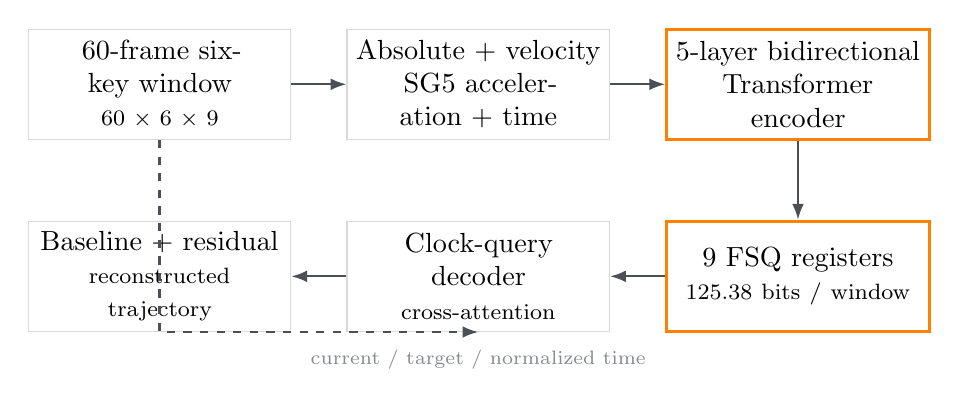
\begin{tikzpicture}[
  box/.style={draw=ArenaLine,fill=white,minimum height=14mm,text width=31mm,align=center},
  accent/.style={box,draw=ArenaPapaya,line width=1.1pt},
  arrow/.style={-{Latex[length=2mm]},draw=ArenaGraphite,line width=.8pt}
]
\node[box] (input) {60-frame six-key window\\\footnotesize $60\times6\times9$};
\node[box,right=7mm of input] (features) {Absolute + velocity\\SG5 acceleration + time};
\node[accent,right=7mm of features] (enc) {5-layer bidirectional\\Transformer encoder};
\node[accent,below=10mm of enc] (latent) {9 FSQ registers\\\footnotesize 125.38 bits / window};
\node[box,left=7mm of latent] (dec) {Clock-query decoder\\\footnotesize cross-attention};
\node[box,left=7mm of dec] (out) {Baseline + residual\\\footnotesize reconstructed trajectory};
\draw[arrow] (input)--(features);
\draw[arrow] (features)--(enc);
\draw[arrow] (enc)--(latent);
\draw[arrow] (latent)--(dec);
\draw[arrow] (dec)--(out);
\draw[arrow,dashed] (input.south) |- (dec.south);
\node[font=\scriptsize,text=ArenaMid,below=1mm of dec] {current / target / normalized time};
\end{tikzpicture}
\caption{两条 Temporal arm 共享 frame encoder 和 residual decoder 的总体形式。}
\end{figure}

\begin{darkbox}{当前验证的是 codec，不是 predictor}
训练随机选择后半段目标帧 $k$，但 encoder 仍然看到完整窗口，包括 $k$ 后的帧；decoder 还显式获得 current、target、$k_{norm}$ 和输出长度。因此当前学习的是
\[
P(\text{discrete motion representation}\mid\text{complete window, endpoints}),
\]
而不是 $P(\text{future}\mid\text{observed prefix, intent})$。
\end{darkbox}

\begin{boundarybox}{Residual prior}
两条 arm 都以 current 到 target 的直线插值作为结构先验，网络只预测偏离该直线的 residual。endpoint-only regression 已能解释运动摘要的中位 $R^2=0.174$；latent 的价值必须以“超出 endpoint 的增量”衡量。
\end{boundarybox}

% ---------------------------------------------------------------- Arms
\section{两条 Temporal arm 学到不同的时间几何}

\begin{minipage}[t]{0.49\linewidth}
\begin{insightbox}{JEPA / 8 path + 1 time}
\begin{itemize}
  \item 8 个 learned queries 全局读取 frame 与 endpoint context。
  \item path registers 无固定时间槽位，是分布式全局表征。
  \item 单独的 time register 读取累计弧长曲线、总路程、帧数比例和平均速度。
  \item JEPA loss 是同 encoder 的 stop-gradient latent reconstruction，并非经典 I-JEPA target encoder。
\end{itemize}
\end{insightbox}
\end{minipage}\hfill
\begin{minipage}[t]{0.49\linewidth}
\begin{insightbox}{MaskFSQ / 9 temporal groups}
\begin{itemize}
  \item warmup 后对 frame token 做 rand / sparse / prefix masking。
  \item 60 帧先分成 9 个固定连续组，并在组内 attention pooling。
  \item 9 个 group token 随后进入 2 层全局 Transformer。
  \item 最终 code 是“时间锚定、全局上下文化”，并非互相独立的局部片段。
\end{itemize}
\end{insightbox}
\end{minipage}

\begin{figure}[H]
\centering
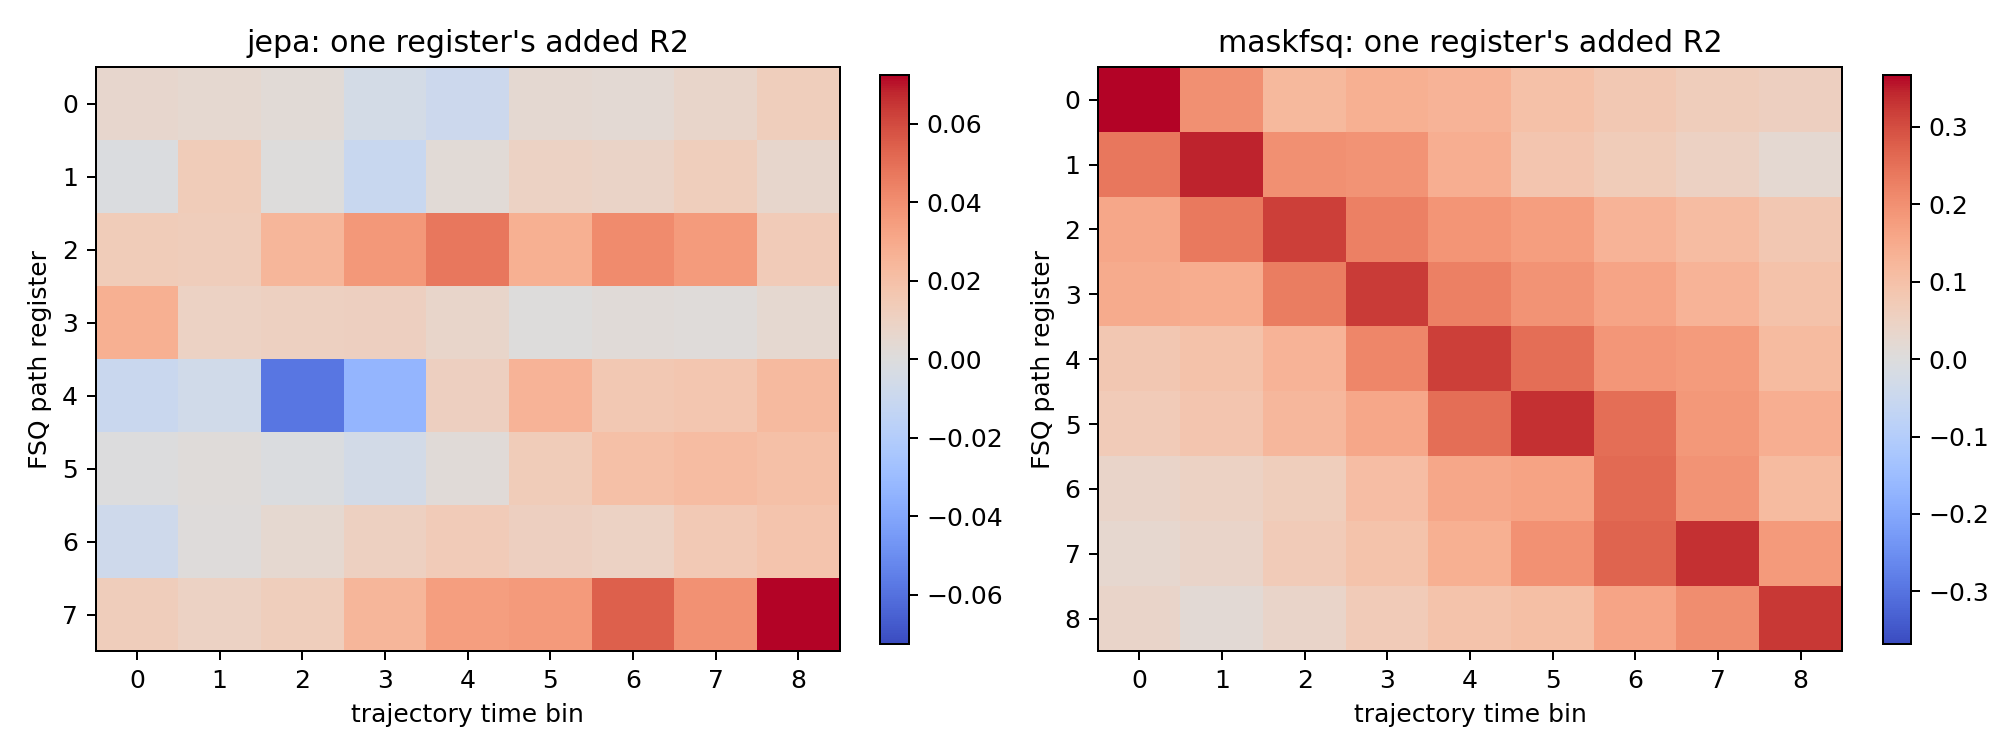
\includegraphics[width=0.96\linewidth]{temporal_locality.png}
\caption{单个 register 对 9 个轨迹时间段的增量 $R^2$。MaskFSQ 显示明显对角带，同时存在跨时间信息扩散。}
\end{figure}

\metric{0.016}{JEPA diagonal added $R^2$}\hfill
\metric{0.011}{JEPA off-diagonal}\hfill
\metric{0.325}{MaskFSQ diagonal}\hfill
\metric{0.135}{MaskFSQ off-diagonal}

% ---------------------------------------------------------------- Factorization
\section{JEPA 的 time register 不是“时长 token”}

\begin{figure}[H]
\centering
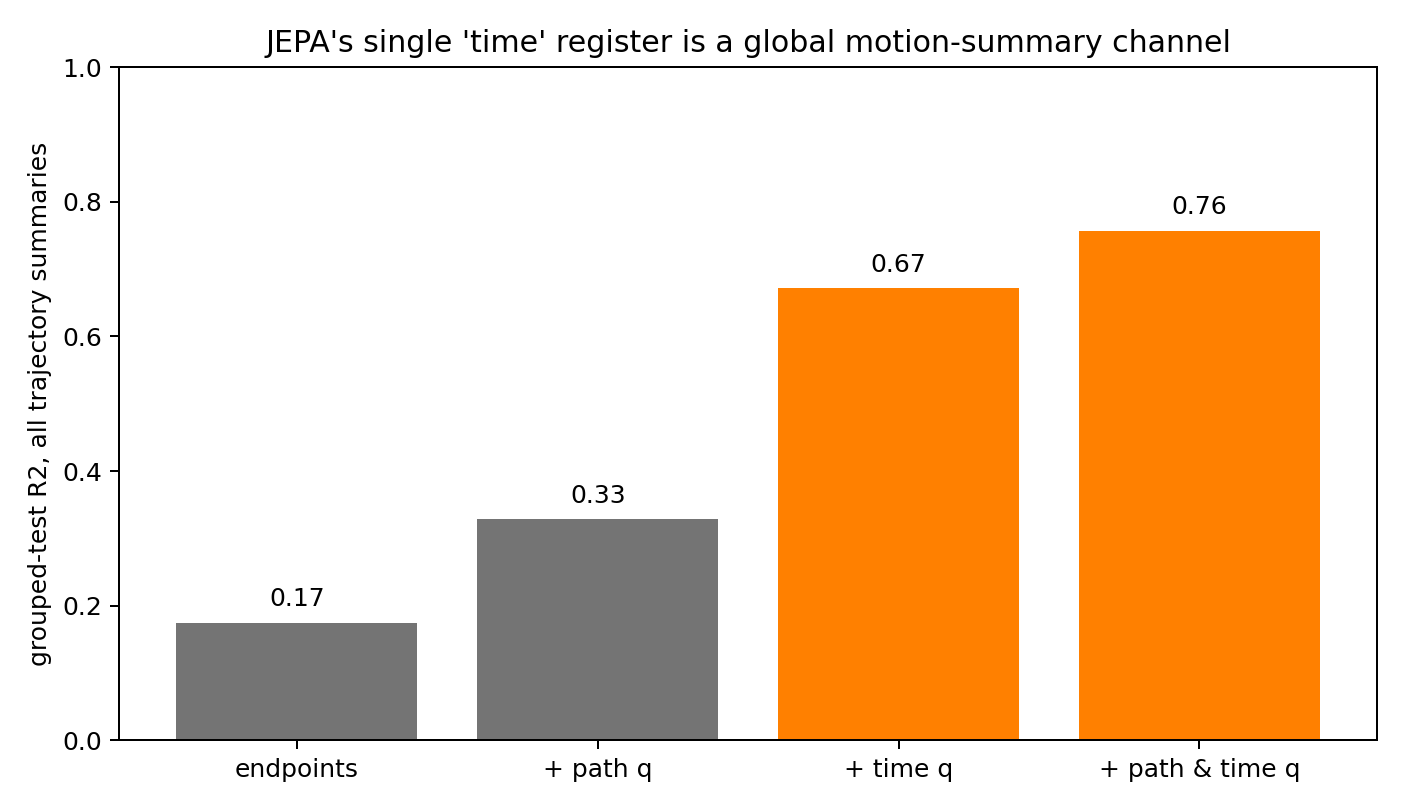
\includegraphics[width=0.82\linewidth]{jepa_factorization.png}
\caption{Grouped ridge 对 33 个轨迹摘要的解释度。time register 本身已经携带大量全局运动信息。}
\end{figure}

\begin{tabularx}{\linewidth}{@{}lR@{}}
\toprule
输入到 linear probe & 轨迹摘要中位 $R^2$ \\
\midrule
Endpoints only & 0.174 \\
Path quantized only & 0.190 \\
Endpoints + path quantized & 0.328 \\
Time quantized only & 0.631 \\
Endpoints + time quantized & 0.671 \\
Endpoints + all quantized latents & 0.757 \\
Endpoints + all continuous latents & 0.780 \\
\bottomrule
\end{tabularx}

\begin{insightbox}{机制解释}
time register 是一条\textbf{粗粒度全局运动摘要通道}。它概括路径进度和运动能量；path bank 则承担无法被这些摘要覆盖的动作细节。两者不是严格的“内容 / 时长”二分。
\end{insightbox}

% ---------------------------------------------------------------- Incremental / causal
\section{相关性之外：decoder 真的使用这些 latent}

\begin{figure}[H]
\centering
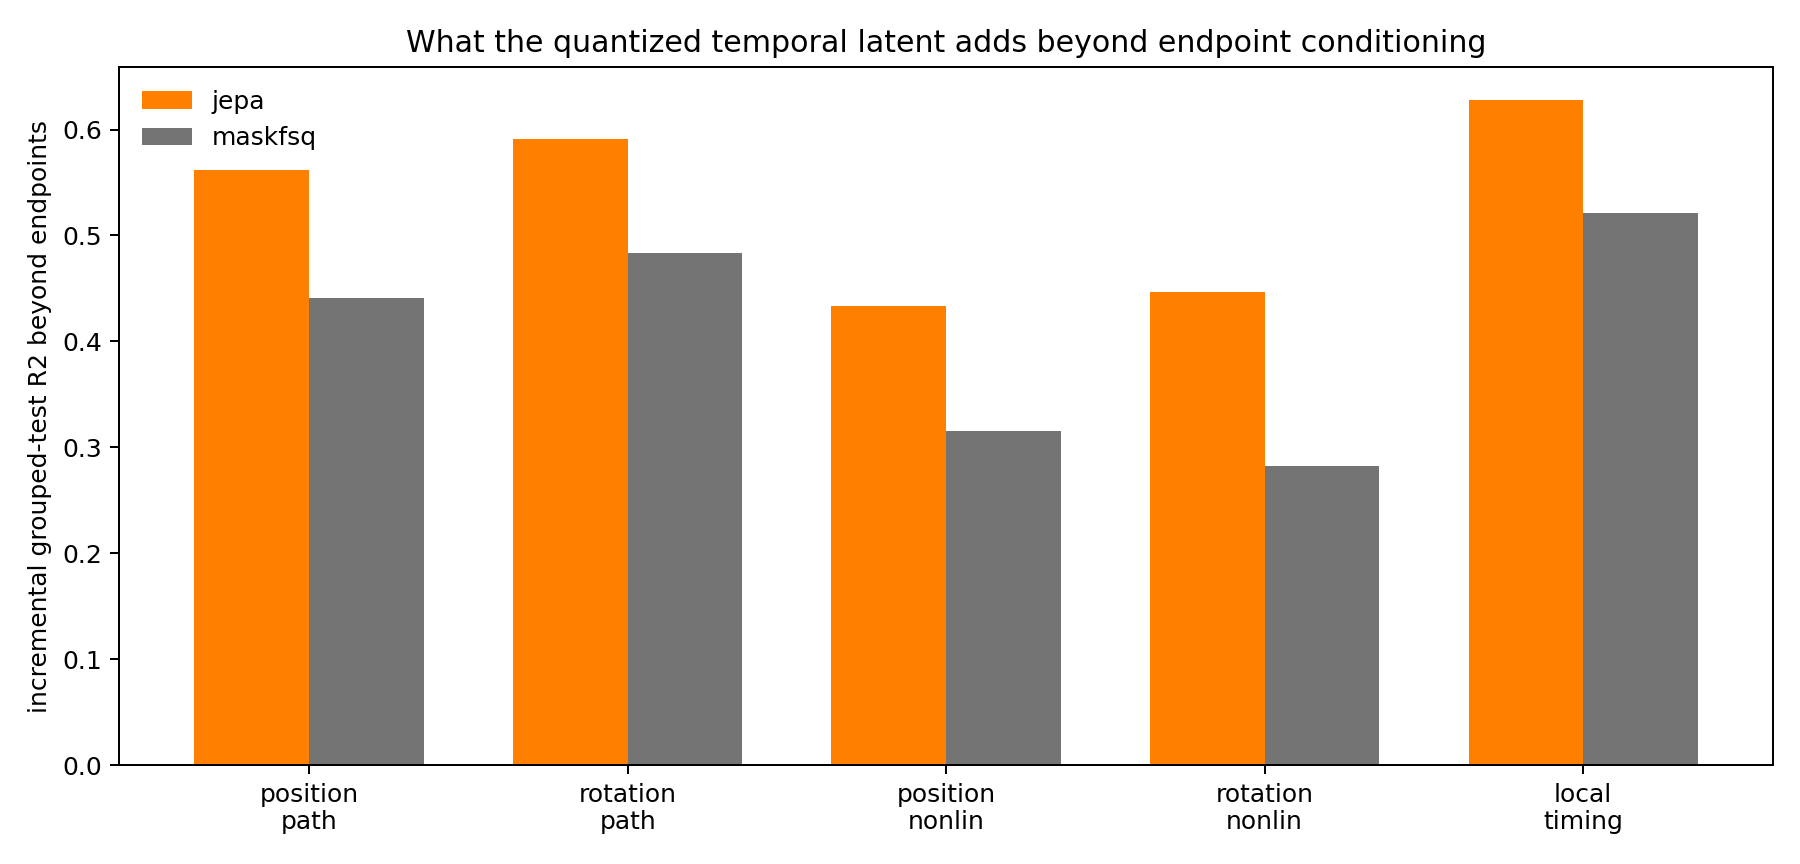
\includegraphics[width=0.98\linewidth]{temporal_incremental_r2.png}
\caption{量化 latent 在 endpoint conditioning 之外增加的 grouped-test $R^2$。}
\end{figure}

\begin{tabularx}{\linewidth}{@{}lYRR@{}}
\toprule
模型 & 因果干预 & 位置误差 & 相对正确 code \\
\midrule
JEPA & 正确 code & 6.743 cm & -- \\
JEPA & 跨样本打乱 path & 11.847 cm & +5.117 cm \\
JEPA & 跨样本打乱 time & 8.598 cm & +1.856 cm \\
MaskFSQ & 正确 code & 6.395 cm & -- \\
MaskFSQ & 跨样本打乱 path & 15.315 cm & +8.925 cm \\
\bottomrule
\end{tabularx}

\vspace{4mm}
\begin{boundarybox}{为什么 shuffle 比 zero 更可信}
跨样本 shuffle 保持 code 在训练分布内，只破坏它与当前动作的对应关系。zero code 属于分布外干预，适合作为 stress test，但不能单独用于解释功能。
\end{boundarybox}

% ---------------------------------------------------------------- Rate
\section{最明确的量化边界：速率方向被 FSQ 抹掉}

\begin{figure}[H]
\centering
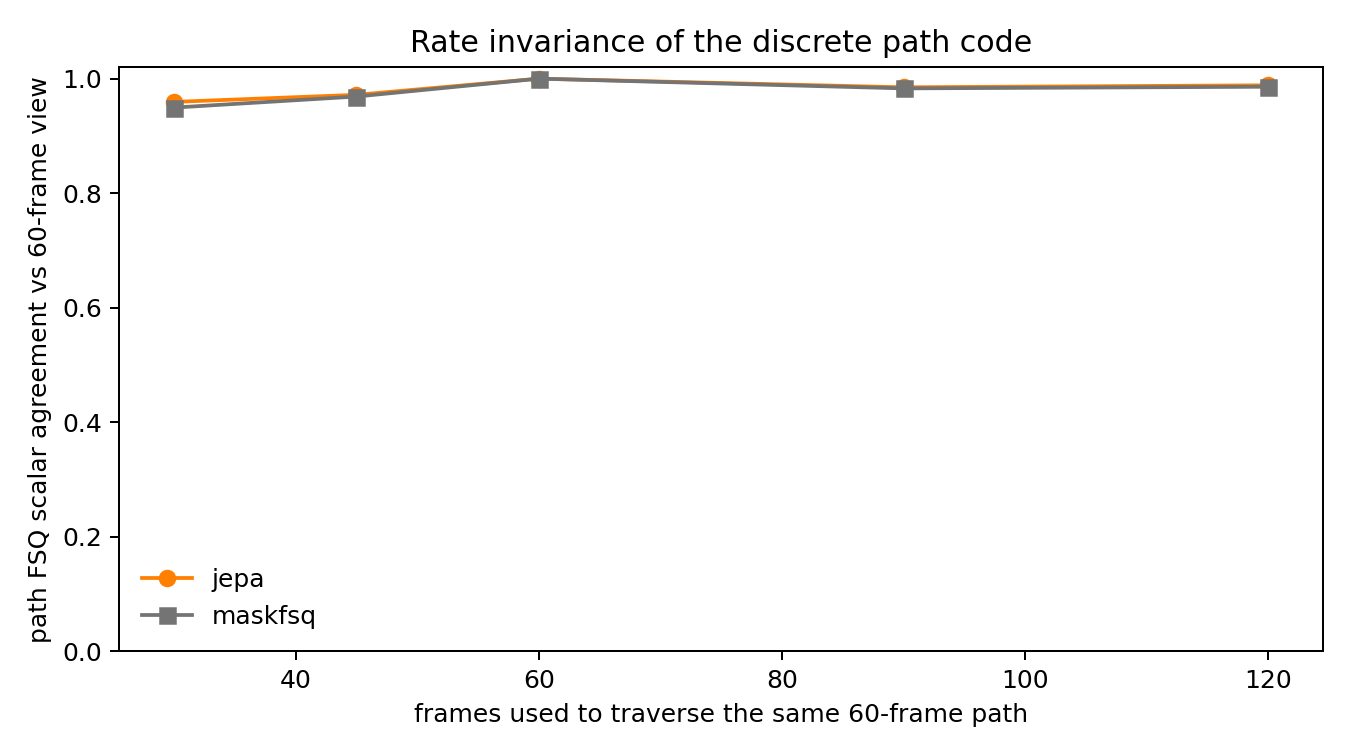
\includegraphics[width=0.82\linewidth]{rate_invariance.png}
\caption{同一路径以 30/45/60/90/120 帧通过时，离散 path code 保持高度一致。}
\end{figure}

\begin{tikzpicture}[x=1mm,y=1mm]
  \fill[ArenaBlack] (0,0) rectangle (174,42);
  \node[anchor=west,text=white,font=\bfseries] at (9,32) {JEPA time feature 中的速率可读性};
  \node[anchor=west,text=ArenaPapaya,font=\fontsize{27}{29}\selectfont\bfseries] at (9,14) {89.7\%};
  \draw[-{Latex[length=3mm]},ArenaPapaya,line width=1.5pt] (62,16)--(102,16);
  \node[anchor=west,text=ArenaPapaya,font=\fontsize{27}{29}\selectfont\bfseries] at (110,14) {23.1\%};
  \node[anchor=west,text=ArenaMid,font=\footnotesize] at (9,6) {continuous $f$};
  \node[anchor=west,text=ArenaMid,font=\footnotesize] at (110,6) {quantized $q$ / chance 20\%};
\end{tikzpicture}

\begin{insightbox}{这不是上游没学到}
连续 time pathway 中存在清晰的线性速率方向；经过当前 6 维、5-level FSQ rounding 后几乎不可读。量化损失是\textbf{方向选择性的}，并非统一降低一点精度。
\end{insightbox}

% ---------------------------------------------------------------- Matched comparison
\section{同样本重建差异：可信，但不能直接归因}

\begin{tabularx}{\linewidth}{@{}lRRR@{}}
\toprule
指标 & JEPA & MaskFSQ & Mask $-$ JEPA，95\% CI \\
\midrule
位置误差 & 6.743 cm & 6.395 cm & $-0.358\ [-0.432,-0.286]$ cm \\
旋转误差 & 10.647$^\circ$ & 9.840$^\circ$ & $-0.811\ [-0.943,-0.684]^\circ$ \\
运动能量保持 & 0.899 & 0.939 & $+0.039\ [+0.032,+0.046]$ \\
\bottomrule
\end{tabularx}

\vspace{7mm}
\begin{darkbox}{不要把这张表写成架构胜负}
两条 arm 不只改变 token geometry。它们同时改变 frame masking、JEPA loss、time register、encoder endpoint context 和 invariance augmentation。匹配 62.69 bit/s 只消除了码率差异，没有形成单变量实验。
\end{darkbox}

\subsection{FSQ 使用情况}

\begin{tabularx}{\linewidth}{@{}lRR@{}}
\toprule
Code bank & 标量独立熵之和 & 名义容量 \\
\midrule
JEPA path & 96.00 bits & 111.45 bits \\
JEPA time & 9.67 bits & 13.93 bits \\
MaskFSQ path & 123.72 bits & 125.38 bits \\
\bottomrule
\end{tabularx}

\smallskip
{\footnotesize\color{ArenaMid}标量熵求和忽略维度依赖，是 joint entropy 的上界，不能直接当作真实压缩率。}

% ---------------------------------------------------------------- Crossbody / data
\section{跨骨架与数据支撑度}

\begin{minipage}[t]{0.48\linewidth}
\begin{darkbox}{Embodiment identity probe}
\begin{tabularx}{\linewidth}{@{}YR@{}}
Endpoint only & 93.1\% \\
JEPA path latent & 25.3\% \\
MaskFSQ path latent & 22.9\% \\
Chance & 20.0\% \\
\end{tabularx}
\end{darkbox}
\end{minipage}\hfill
\begin{minipage}[t]{0.48\linewidth}
\begin{insightbox}{解释}
Temporal cross-body InfoNCE 显著压低了身体身份，但没有完全消除。机器人间 CKA 高于 human-to-robot，部分来源是它们共享同一 retargeting pipeline，不能单独当作自然跨形态泛化证据。
\end{insightbox}
\end{minipage}

\begin{figure}[H]
\centering
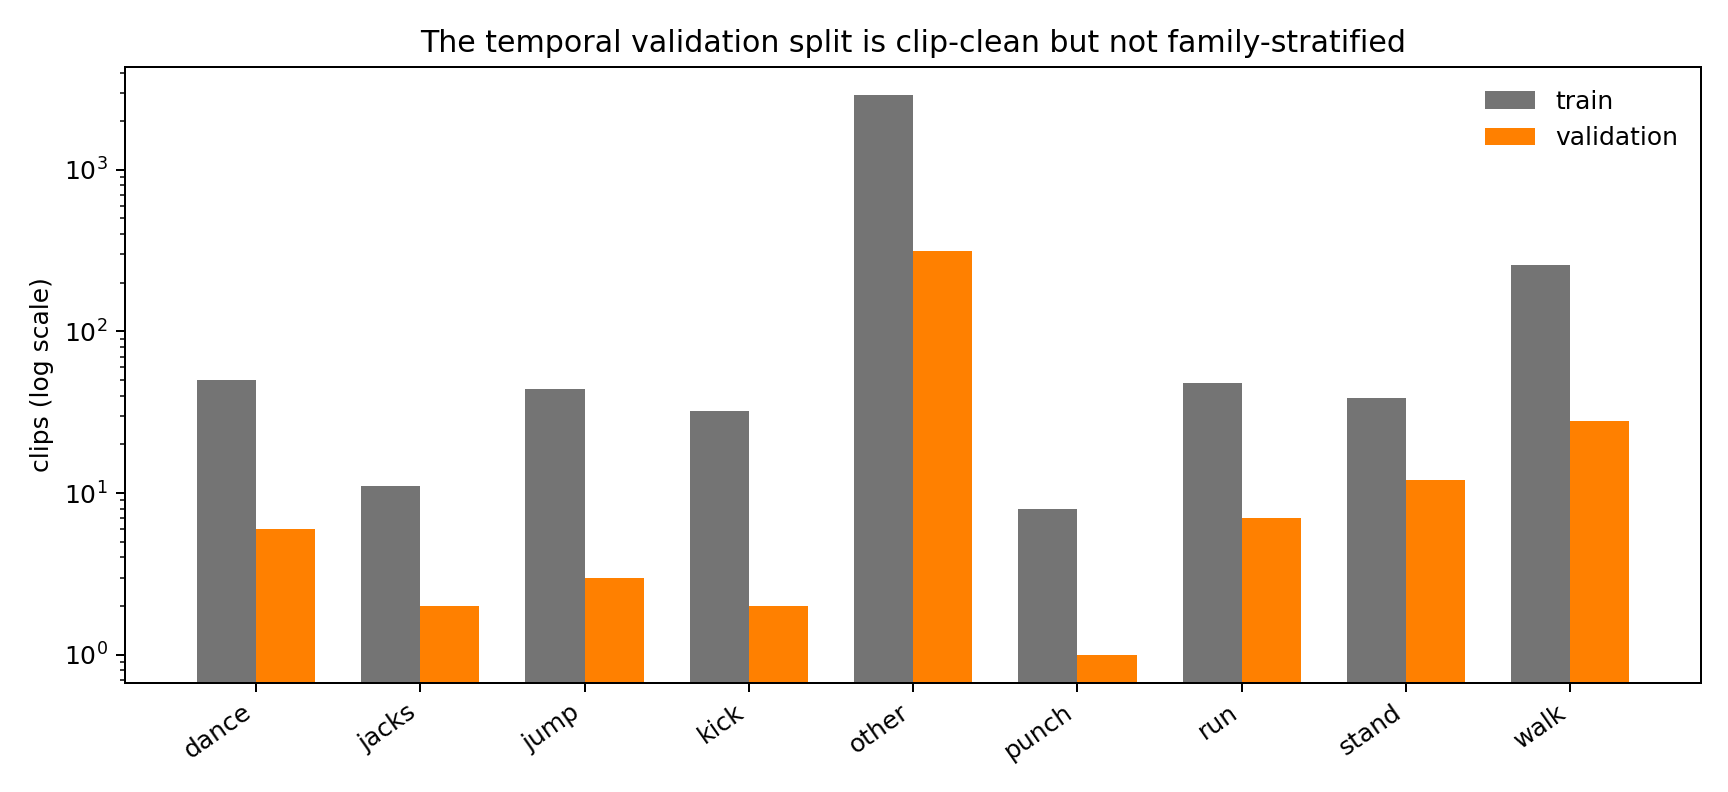
\includegraphics[width=0.92\linewidth]{data_split_support.png}
\caption{Temporal clip-level split 的动作族支撑。验证集未按 family 分层，稀有动作的结论不稳定。}
\end{figure}

\begin{boundarybox}{评估协议的三处风险}
\begin{enumerate}
  \item Spatial 旧评估使用 frame-level random split，相邻帧可能跨 train / val；本文 Spatial probe 改用 AMASS，避免直接复用该 split。
  \item Temporal 是 clip-clean split，但 punch 仅 1 个 val clip，kick 和 jacks 各 2 个，jump 3 个。
  \item family probe 只说明训练分布中存在可线性读取的类别结构，不是组合泛化或 OOD 理解证据。
\end{enumerate}
\end{boundarybox}

% ---------------------------------------------------------------- Evidence boundary
\section{证据边界：现在可以说什么}

\begin{minipage}[t]{0.49\linewidth}
\begin{insightbox}{\textcolor{ArenaGreen}{已有证据支持}}
\begin{itemize}
  \item Spatial 形成共享但带身体签名的姿态流形。
  \item Temporal 以约 62.69 bit/s 保留路径、非线性和局部时序信息。
  \item JEPA 是全局分布式表示；MaskFSQ 是时间锚定、全局上下文化表示。
  \item FSQ 对不同信息方向有选择性损失。
  \item latent 对 decoder 输出具有因果作用。
\end{itemize}
\end{insightbox}
\end{minipage}\hfill
\begin{minipage}[t]{0.49\linewidth}
\begin{insightbox}{\textcolor{ArenaRed}{目前不能宣称}}
\begin{itemize}
  \item Spatial hidden state 被 Temporal 直接建模。
  \item Temporal 已能只看过去生成未来。
  \item JEPA 或 MaskFSQ 已经胜出。
  \item token 具有固定的人类可读动作语义。
  \item 系统已学到 contact-aware、physics-solid 闭环控制。
\end{itemize}
\end{insightbox}
\end{minipage}

\begin{darkbox}{物理边界}
默认 \code{root\_vel=False}；位置均为 root-relative。当前输入和损失中没有 world translation、contact、IMU、torque 或 actuator state。现有数字衡量的是运动表示与运动学重建，不是 WBC 的稳定性、柔顺性和抗扰恢复。
\end{darkbox}

% ---------------------------------------------------------------- Experiments
\section{下一轮最小可归因实验矩阵}

\begin{tabularx}{\linewidth}{@{}p{9mm}p{50mm}Y@{}}
\toprule
编号 & 控制变量 & 要回答的问题 \\
\midrule
01 & 固定 token geometry，只开/关 frame masking & 局部结构收益来自 token 位置，还是来自遮挡训练？ \\
02 & 固定 token geometry，只开/关 JEPA loss & stop-gradient target 是否真正改变表示几何？ \\
03 & 固定 encoder context，只开/关 time register & 全局摘要通道是否必要，是否挤占 path capacity？ \\
04 & 两条 arm 使用相同 invariance augmentation & 当前 warp / uniform 差异贡献多少？ \\
05 & prefix-only causal encoder，移除 acausal SG 特征 & 模型是否能从已观测历史预测未见未来？ \\
06 & family-stratified clip split & 稀有动作结果是否可复现？ \\
07 & 分开测 Temporal six-key 与 Spatial completion error & 两层分别贡献多少误差？ \\
08 & 加入 world root、contact、IMU 与 WBC rollout & 表示质量是否转化为真实物理执行能力？ \\
\bottomrule
\end{tabularx}

\vfill
\begin{tikzpicture}[x=1mm,y=1mm]
  \fill[ArenaPapaya] (0,0) rectangle (174,1.5);
  \node[anchor=west,font=\bfseries] at (0,-7) {研究原则};
  \node[anchor=west,text width=145mm,font=\small,text=ArenaGraphite] at (26,-7)
    {先构造可归因的反事实，再讨论架构选型；先区分运动学、动力学与控制，再讨论“physical intelligence”。};
\end{tikzpicture}

% ---------------------------------------------------------------- Appendix
\newpage
\section*{附录：可复现资产与方法}
\addcontentsline{toc}{section}{附录：可复现资产与方法}

\begin{tabularx}{\linewidth}{@{}p{37mm}Y@{}}
\toprule
资产 & 路径 / 方法 \\
\midrule
完整机器可读结果 & \path{pose_translator_design/audits/DEEP_AUDIT_0807/audit.json} \\
审计脚本 & \path{pose_translator_design/exp_topo/audit_spatiotemporal_latent.py} \\
Temporal 抽样 & 1,494 unique windows / 376 validation clips / max 4 windows per clip \\
回归 & clip-grouped Ridge；报告 grouped-test median $R^2$ \\
区间估计 & paired clip bootstrap，95\% interval \\
因果干预 & in-distribution cross-sample latent shuffle；zero code 仅作 OOD stress test \\
Spatial probe & 240 AMASS frames / 5 embodiments；独立于 E19 的 LAFAN frame split \\
模型状态 & checkpoints read-only；无参数更新，无重新训练 \\
\bottomrule
\end{tabularx}

\vspace{12mm}
\begin{darkbox}{审计对象}
\code{E19\_K128\_0805} \quad / \quad
\code{V7\_jepa\_0807} \quad / \quad
\code{V7\_maskfsq\_0807}
\end{darkbox}

\vfill
\begin{center}
\includegraphics[width=13mm]{../../../alpha_motion2/assets/brand/apocynthion-mark-papaya.png}\par
\vspace{3mm}
{\bfseries ArenaLabs}\par
{\small\color{ArenaMid}Physical AI Research}
\end{center}

\end{document}
